\newpage
\section{2D System Simulation}
As it is mentioned earlier, the whole idea of the project is to make the antenna of the drone and the ground stations point at each others. To achieve this its needed to know the angle of the antennas and their optimal angle, which is when they point exactly at each others. To be able to point the antennas towards each others two controllers will be implemented. In this section an algorithm to calculate the optimal angle will be introduced. Furthermore the implementation of the controllers will be explained.
\subsection{Scenario}
In Figure \ref{fig:drone_gs} it is shown a scenario where the antennas of both GS and drone change after some periods of time. In the top part of the figure it shows the angle of the drone ($\theta_{d}$) and the optimal angle ($\theta_{opt\_d}$) that the antenna want to be in. In the lower part of the figure it shows the angle of the ground station ($\theta_{gs}$) and the optimal angle ($\theta_{opt\_gs}$). 

\begin{figure}[h]
	\centering
	
	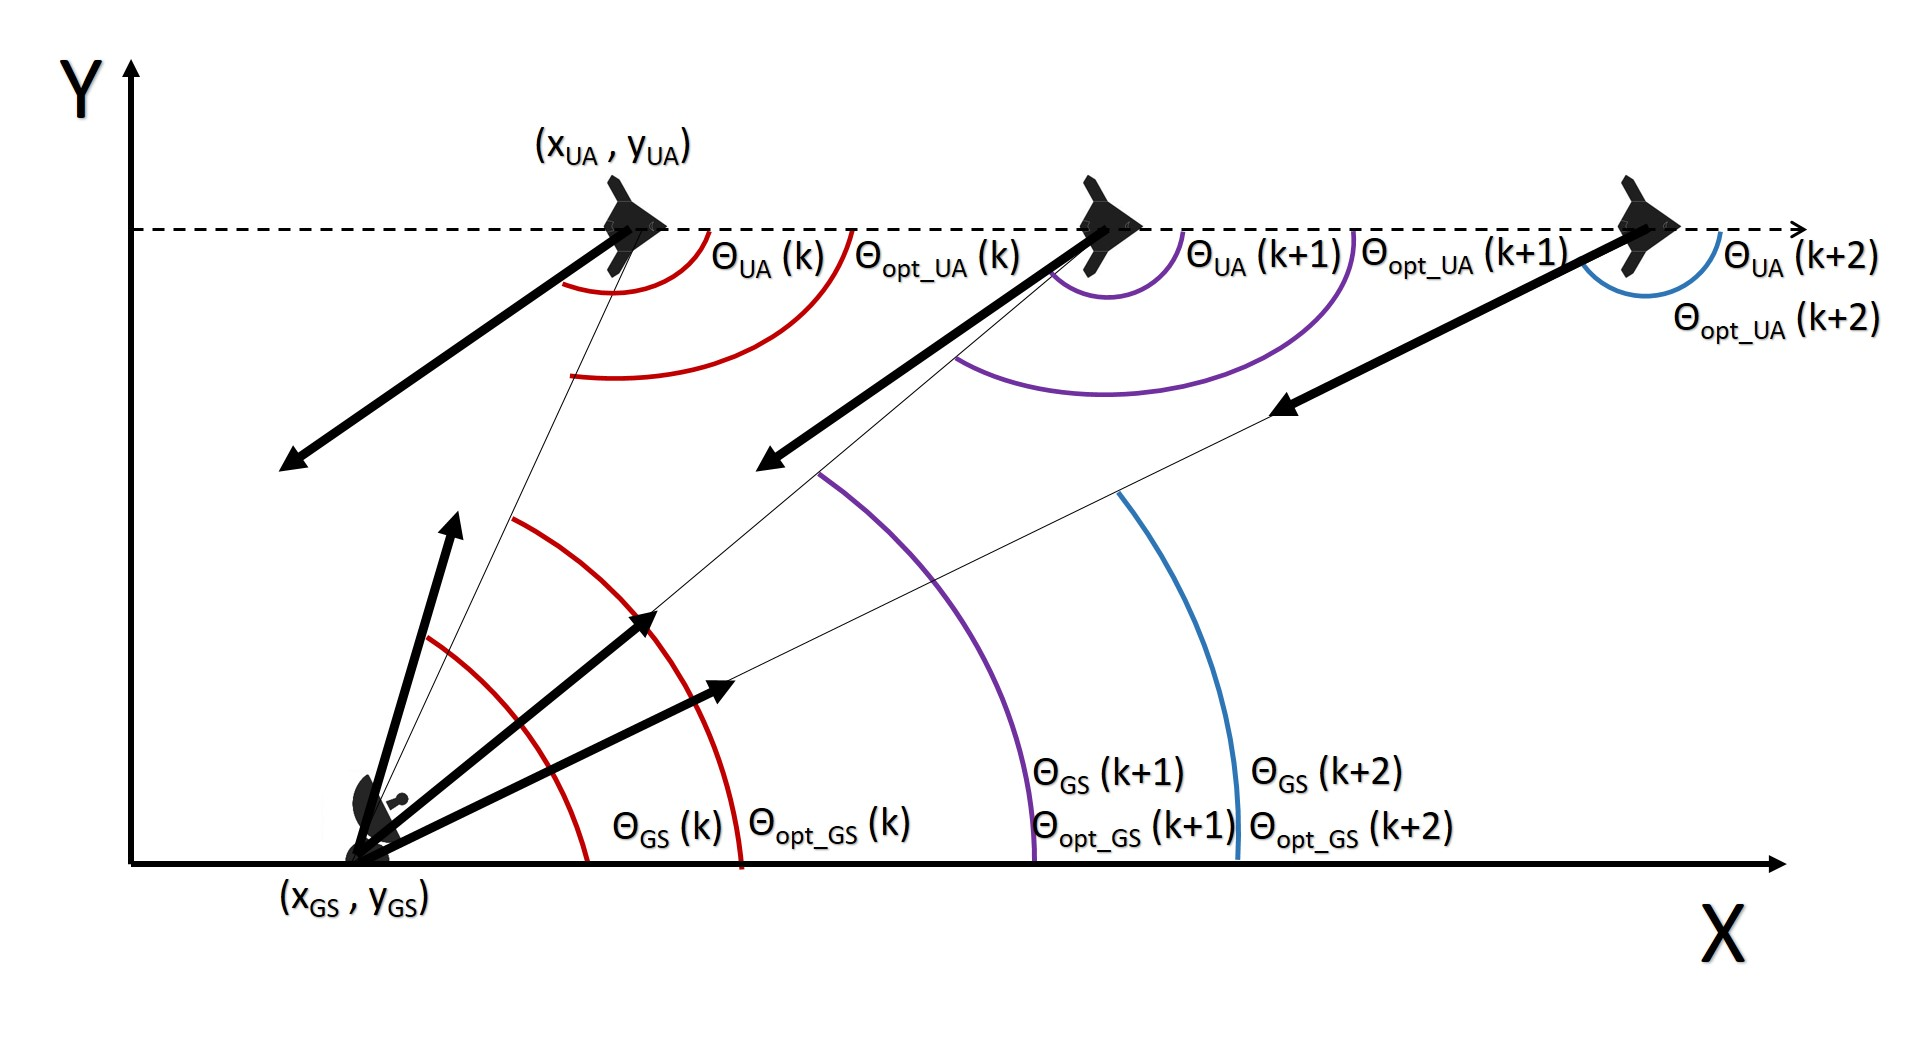
\includegraphics[scale=0.45]{figures/drone_gs_ex_1.jpg}
	\caption{Example of a drone-gs scenario}
	\label{fig:drone_gs}
\end{figure}

As it is seen on the figure at time k the antenna of the drone ($\theta_d (k)$) is not equal the optimal angle ($\theta_{opt\_d}(k)$). The same goes with the $\theta_{gs}(k)$ and the optimal angle $\theta_{opt\_gs}(k)$. As the drone moves further on the X-axis the angle of the ground station and the drone goes closer to the optimal angle. 

\subsection{System overview}
The system presented is a Multiple Input Multiple Output (MIMO) system, such that in this case there are 4 inputs and 2 outputs. The system is shown in figure \ref{fig:2d_system}. 

\begin{figure}[h]
	\centering
	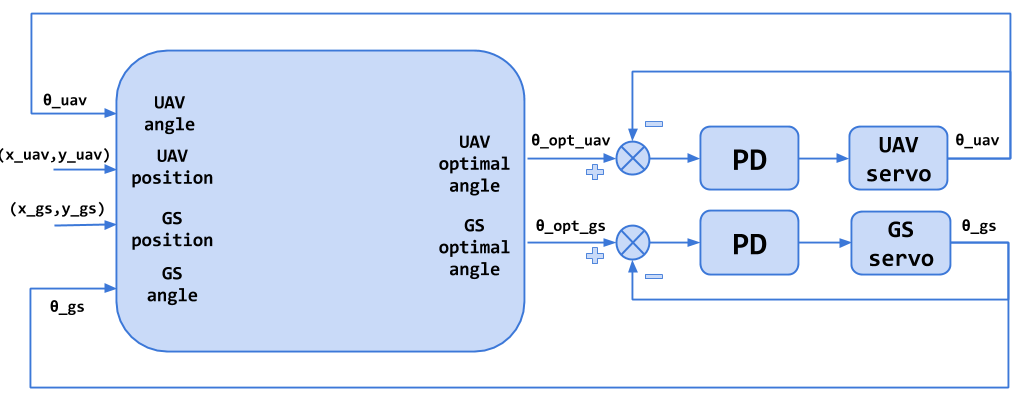
\includegraphics[scale=0.42]{figures/2d_system.png}
	\caption{2D sytem overview}
	\label{fig:2d_system}
\end{figure}
The first block of the system takes as inputs the parameters below and computes the optimal angles for the ground station ($\theta\_opt\_gs$) and drone ($\theta\_opt\_d$) antennas, such that a strong communication link is achieved. \\

\noindent The 2 outputs, of the first block, that it is needed to control are:
\begin{itemize}
	\item Drone's antenna angle ($\theta_{d}$)
	\item Groundstation's antenna angle ($\theta_{gs}$)
\end{itemize}

\noindent The system's inputs are as follows:
\begin{itemize}
	\item Drone's antenna angle ($\theta_{d}$)
	\item Groundstation's antenna angle ($\theta_{gs}$)
	\item Drone position ($x_{drone},y_{drone}$)
	\item Groundstation position ($x_{gs},y_{gs}$)
\end{itemize}

\subsection{Optimal angle}
The right part of figure \ref{fig:2d_system} shows two PD controllers where each of them have a servomotor connected. The PD controller is explained in chapter \ref{dcmotor_circuit} and the servo is explained in chapter \ref{ch:simulation}. The left block have two output which is $\theta\_opt\_d$ and $\theta\_opt\_gs$. They are the optimal angle that the drone and ground station need to have to be pointing at each other (Figure \ref{fig:drone_gs}). The PD controllers purpose is to make the servomotors rotate the antenna to the correct position. The PD controllers take the error ($\theta\_opt\_d$ -$\theta\_d$) for the drone and ($\theta\_opt\_gs$ - $\theta\_gs$ for the ground station, and make the servomotors rotate the antenna to the correct position. When the error is zero, which means the input to the PD controller is zero, the antennas are at the correct angles.   

\subsection{Simulations}
To verify that the 2D simulations work, some simulations are made. In the first simulation the drone is simulated by starting in (0,50) and going to (100,50), which means that the drone is only moving in the x-axis. The simulation is shown in figure \ref{fig:gs_angle_vs_optimal} where the top one is showing the Drone angle versus the optimal angle and the bottom one is showing the ground station angle versus the optimal one. 

\begin{figure}[h]
	\centering
	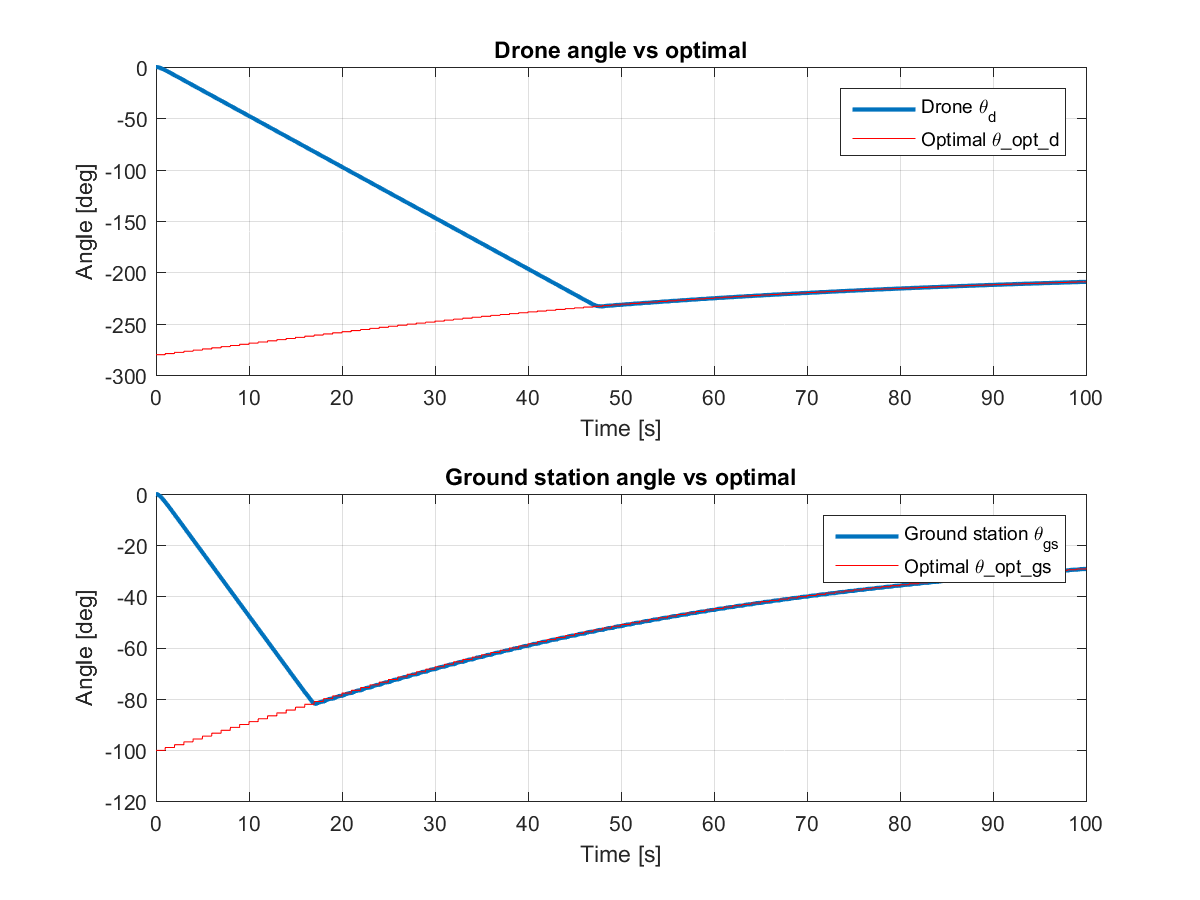
\includegraphics[scale=0.6]{figures/gs_angle_vs_optimal.png}
	\caption{Ground station angle vs optimal}
	\label{fig:gs_angle_vs_optimal}
\end{figure}

In this plot the angle is shown in degree to make it easier to understand. The blue line in both plots is respectively the drone and the ground stations antenna angle. They both start in 0 degree and have no initial starting point. Here it takes about 46 seconds for the drones antenna to be at the optimal angle and in the other case it takes about 17 seconds for the ground station antenna to turn to the optimal angle. But when they reached their optimal angle, the controller holds the antennas to the optimal angle. 
\newpage
